\documentclass[aspectratio=169]{beamer}              % only frames

% for themes, etc.
\mode<presentation>
\usetheme{Madrid} 
\usecolortheme{crane}

%\usepackage{times}  % fonts are up to you
% The usual suspects
\usepackage{multirow, booktabs, dcolumn, color, graphicx} % Tables\usepackage{graphicx}
\usepackage{amsmath,amssymb,amsthm}
% Strikethrough text
\usepackage{soul}
% Adjust box to fit tabulars
\usepackage{adjustbox}
% Embed video
\usepackage{media9}
% For notes
\usepackage{pgfpages}
\setbeameroption{hide notes} % Only slides
%\setbeameroption{show only notes} % Only notes
%\setbeameroption{show notes on second screen=right} % Both
% Use colors by name
\usepackage{xcolor}
% EMBEDDING VIDEO IS POSSIBLE WITH PDFPC USE PDF PC to present
\usepackage{multimedia}



% The table highlighting for hypothesis discussion.
\usepackage[beamer,customcolors]{hf-tikz}
\usetikzlibrary{calc}

% To use background images
\newenvironment{colorframe}[2][]{%
\setbeamercolor{background canvas}{bg=#1}
\begin{frame}\color{white}}
{\end{frame}}


% To set the hypothesis highlighting boxes red.
\tikzset{hl/.style={
    set fill color=red!80!black!40,
    set border color=red!80!black,
  },
}

% Set Graphics folder
\graphicspath{{./figures/}}


% these will be used later in the title page
\title{Threatlandscape}
\subtitle{Access: Vulnerabilities}
\author{Irfan Kanat}
\institute[CBS]{{Department of Digitization}\\ Copenhagen Business School}
%\date{\today}



\begin{document}

% this prints title, author etc. info from above
\begin{frame}

    \titlepage


    \vfill
    {\tiny \centering This work is licensed under a \href{http://creativecommons.org/licenses/by/4.0/}{Creative Commons Attribution 4.0 International License}.}

\end{frame}

\note{In this presentation we focus on how malicious actors gain access to information assets.}

\begin{frame}
    \frametitle{Big Question}
    
    \large How do they gain access?

\end{frame}

\note{Now that we know who all is out there, let us take a look at how they do what they do.

According to DBIR 2021 report, 85\% of the breaches involved some sort of human involvement. 61\% of the breaches involved credentials.}


\begin{frame}
    \frametitle{Vulnerabilities}
    
    Configuration Errors \vspace{1em}

    Bugs \vspace{1em}

\end{frame}

\note{While credentials are a convenient way to gain access, they are not the only way.

Another way of gaining access is to exploit the vulnerabilities in the systems themselves.

The vulnerability may be misconfiguration of the system. Such as leaving default passwords unchanged, allowing backwards compatibility to older protocols, and so on.

The bugs are errors in the code, that allow a malicious actor to force the system to behave in ways it is not supposed to behave.

Often the bugs and vulnerabilities will come with a way to exploit them. This may be an exploit code, like those found in metasploit framework. Or be embedded in some malware like ransomware that uses these vulnerabilities to propagate through the network.

By exploiting the vulnerability the malicious actors can crash, run arbitrary code on, or escelate their privileges on a system.

You may hear about the 0day, a 0day is a vulnerability that is not yet publicly known and is freely exploitable. Once a vulnerability is discovered, developers rush to develop updates to their software to patch it. An unknown vulnerability will not be patched until it is made known to the developers and is therefore is a very valuable asset.
}


\begin{frame}
    \frametitle{Vulnerabilities: How Bad Can It Be Really?}

    \centering
    
    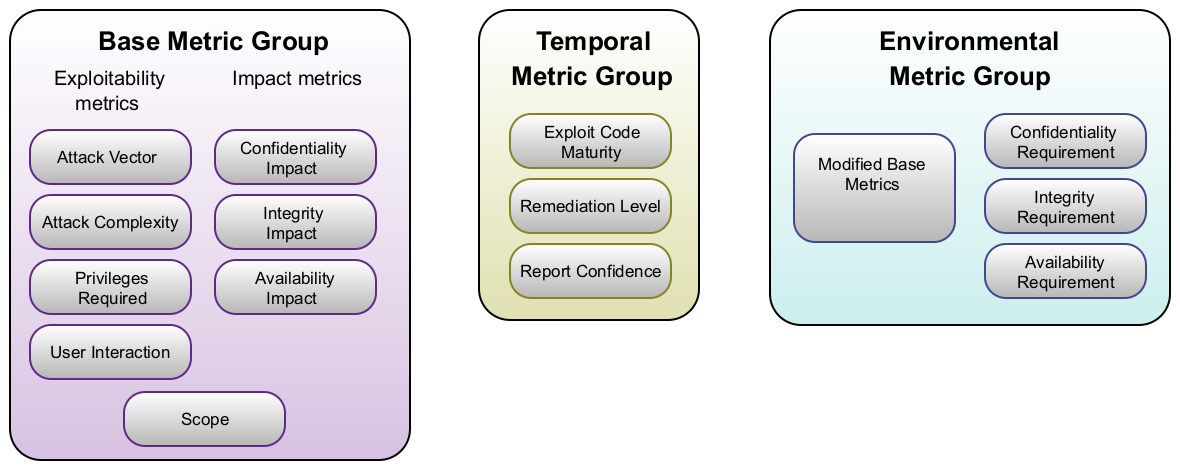
\includegraphics[width = \textwidth, height = .85\textheight, keepaspectratio]{figures/MetricGroups.png}

\end{frame}

\note{How bad the vulnerability depends on a number of factors.

For example a vulnerability that requires a legitimate user to do something (like click a link, run a program) will be less severe than one that doesn't require any user interaction.

A vulnerability that can be exploited remotely will be more severe than one that requires physical access.

Availability of exploit code in the wild will make the vulnerability more severe. While official patch will make it less severe.}

\begin{frame}
    \frametitle{Closing the Vulnerabilities}
    
        \begin{columns}
            \begin{column}{0.5\textwidth}
    
                Update your software \vspace{1em}

                Update your operating system \vspace{1em}

                Update your firmware \vspace{1em}

                Update your anti-malware solutions
        
            \end{column}
    
            \begin{column}{0.5\textwidth}
    
                Remove superfluous software  \vspace{1em}

                Remove unused user accounts \vspace{1em}

                Close unused ports \vspace{1em}
    
            \end{column}
    
        \end{columns}


\end{frame}

\note{
    Whether you are a big organization or a high-school student it is good advice to keep your systems up to date. 

    Another consideration is to reduce the attack surface. Remove the software, accounts, and ports that are not strictly necessary for the functioning of the system. Each additional piece of software is a potential hotbed of bugs and vulnerabilities.

    For corporations there may be additional controls that are viable such as air-gaping critical systems, or monitoring network traffic.
}



\end{document}
